\documentclass{article}

\title{Prototype Forcing File Generator}
\author{Matthew Russell}
\date{February 12 2013}


% Define stuff to use for the title page.
% copied from some french dude...
% I modified it to get it to work

\def\blurb{
  Carleton University \\
  Department of Civil and Environmental Engineering \\
  Faculty of Engineering \\[1em]
}

\def\clap#1{\hbox to 0pt{\hss #1\hss}}%

\newcommand{\cligne}[1] {
	\hbox to \hsize{
		\vbox{\centering #1}
	}
}

\newcommand{\iligne}[1] {
	\hbox to \hsize{
		\vbox{\hspace{23em} #1}
	}
}

\def\haut#1#2#3{
	\hbox to \hsize{
		\rlap{\vtop{\raggedright #1}}
		\hss
		\clap{\vtop{\centering #2}}
		\hss
		\llap{\vtop{\raggedleft #3}}
	}
}

\def\bas#1#2#3{
	\hbox to \hsize{
		\rlap{\vbox{\raggedright #1}}
		\hss
		\clap{\vbox{\centering #2}}
		\hss
		\llap{\vbox{\raggedleft #3}}
	}
}


\newcommand{\ec}{Environment Canada}
\newcommand{\saprc}{SAPRC-07A}
\newcommand{\gm}{\textsc{GEM-MACH}}
\newcommand{\ozone}{O$_3$~}
\newcommand{\no}{NO~}
\newcommand{\nox}{NO$_x$}
\newcommand{\aurams}{\textsc{AURAMS}}
\newcommand{\cmaq}{\textsc{\small{cmaq}}}
\newcommand{\spi}{\textsc{\small{spi}}}
\newcommand{\fortran}{\textsc{Fortran95}}
\newcommand{\fortrankk}{\textsc{Fortran2003}}
\newcommand{\rodas}{\emph{Rodas-3}}
\newcommand{\librmn}{\emph{librmn.a}}
\newcommand{\openmp}{OpenMP}
\newcommand{\ie}{i.e.}
\newcommand{\eg}{e.g.}

\newcommand{\code}[1]{\small{\texttt{#1}}}

% Acronyms
\usepackage[printonlyused,withpage]{acronym}
\acrodef{cmc}[CMC]{\textsc{Canadian Meteorological Centre}}
\acrodef{cam}[CAM]{\textsc{Canadian Aerosol Module}}
\acrodef{kpp}[KPP]{\textsc{Kinetic PreProcessor}}
\acrodef{nrc}[NRC]{\textsc{National Research Council}}
\acrodef{scm}[SCM]{\textsc{Source Control Management}}
\acrodef{svn}[SVN]{\textsc{Subversion}}
\acrodef{tlm}[TLM]{\textsc{Tangent Linear Model}}

% Set the margins to something like 1"
\addtolength{\hoffset}{-1cm}
\addtolength{\textwidth}{2cm}

%\addtolength{\voffset}{-1cm}
\addtolength{\textheight}{2cm}

\usepackage{minted}

% Colours...
\usepackage[pdftex]{hyperref}
\hypersetup{
    colorlinks,
    citecolor=black,
    filecolor=black,
    linkcolor=black,
    urlcolor=blue
}
\usepackage{color}

% Highlight
\usepackage{soul}

% Math stuff
\usepackage{amsthm}
\usepackage{amsmath}
\usepackage{amssymb}

% Fancy enumerate
\usepackage{enumerate}

% Ability to include other PDF documents
\usepackage{pdfpages}

\begin{document}

\maketitle

\section{Proposed Archetecture}

\begin{figure}
	\centering
	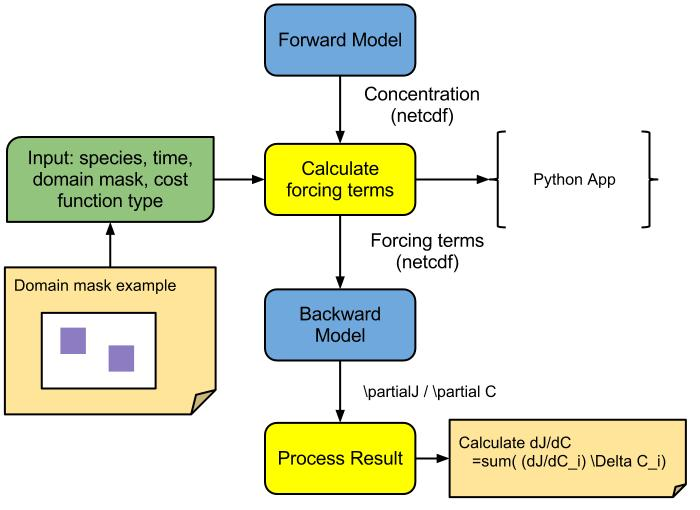
\includegraphics{CMAQ-Adjoint-Process.jpg}
\end{figure}


\begin{figure}
	\centering
	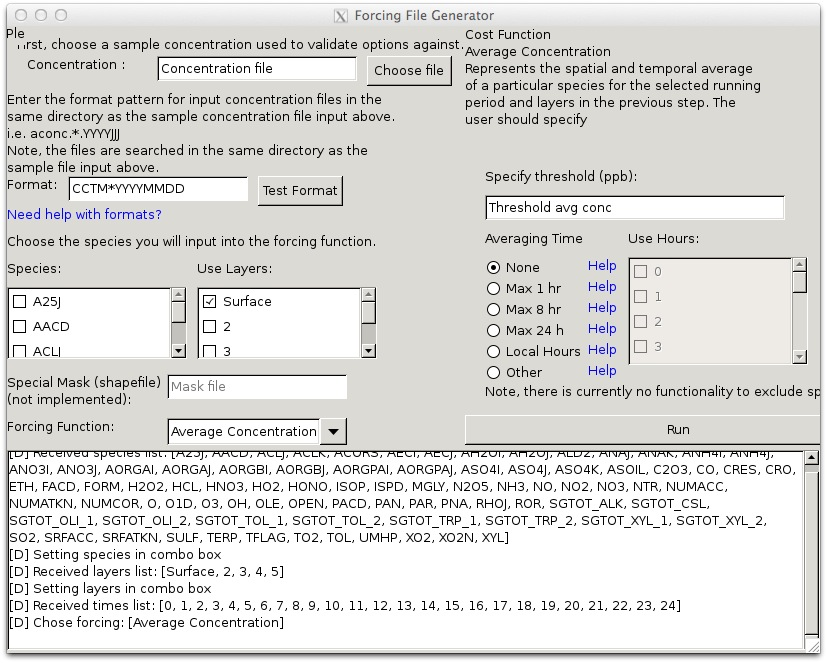
\includegraphics{Forcing_App_Layout-filled.jpg}
\end{figure}

\begin{figure}
	\centering
	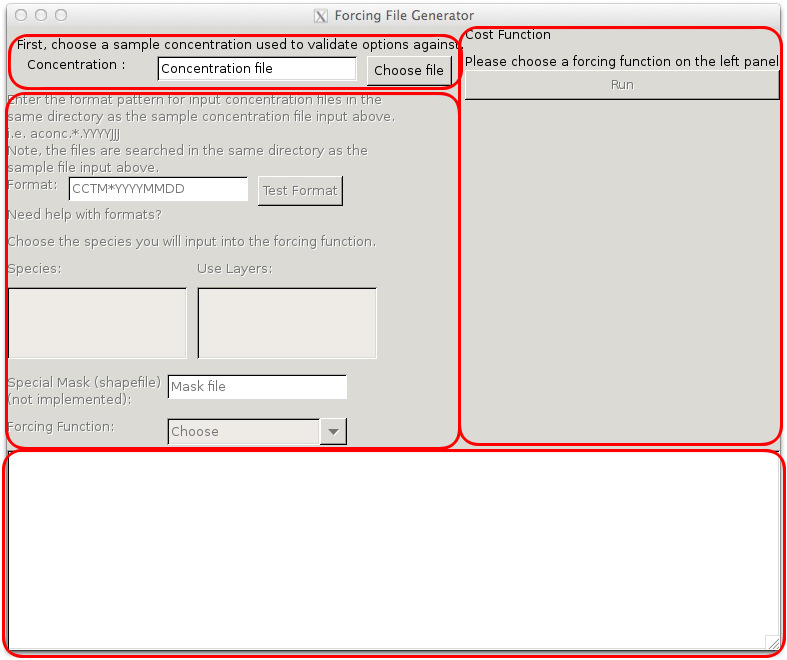
\includegraphics{Forcing_App_Layout.jpg}
\end{figure}

\begin{figure}
	\centering
	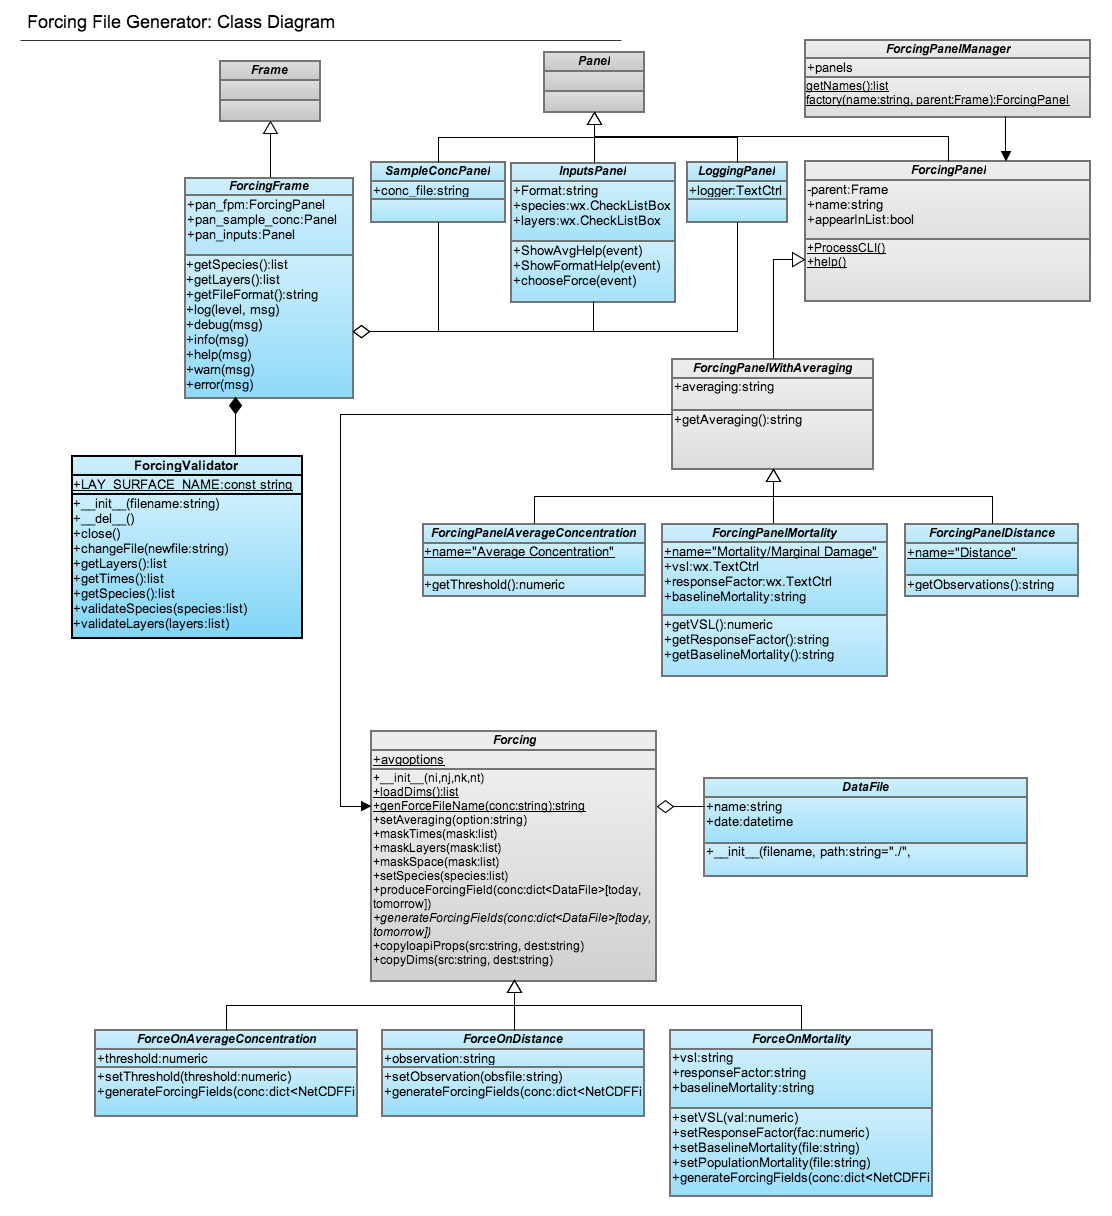
\includegraphics{Forcing_Generator.png}
\end{figure}

\begin{figure}
	\centering
	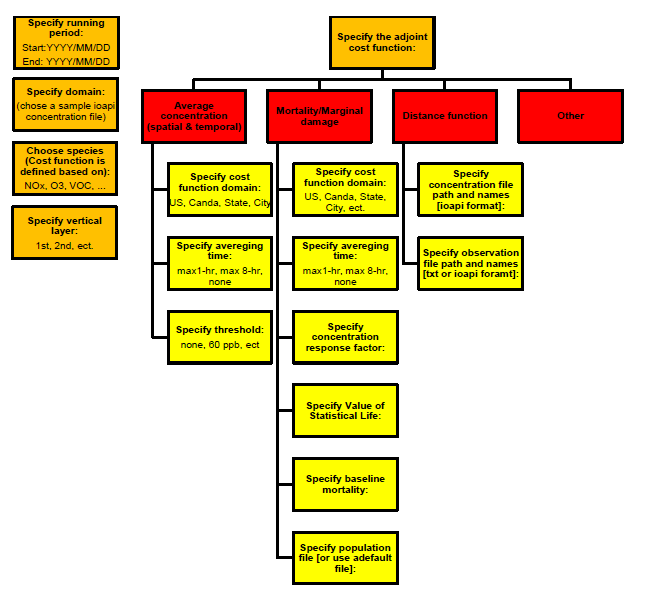
\includegraphics{Forcing-Interface-Chart.png}
\end{figure}

\end{document}
